\newpage
\section{Полученные результаты}
\subsection{Рассчёты в 1D}
Для одномерной модели сплошной среды были реализованы рассчёты линейно-упругой и пластической реологии, движение сетки со вторым порядком точности по времени, получена ударная волна, а также исследован неявный метод второго порядка точности.
\subsubsection{Линейная упругость}
\subparagraph{Неподвижная сетка}
На неподвижной сетке был реализован метод второго порядка по координате, основанный на аппроксимации инвариантов Римана по трём точкам. Рассчёт по данному методу не учитывает движение тела в направлении вдоль колебаний, и может быть применён только в случае малости скоростей или моделировании поперечных колебаний. На      
рис.\ref{pic:el-non-mv} показана скорость частиц тела в разные моменты времени, в том числе после отражения от жёстко закреплённой границы (граничное условие $v = 0$, скорость изменяет знак).

В отличие от метода первого порядка, данный в сочетании с лимитером "minmax" даёт значительно меньшее размытие волнового фронта, при этом осцилляций практически не возникает.

\begin{figure}
\begin{minipage}[h]{0.47\linewidth}
\center{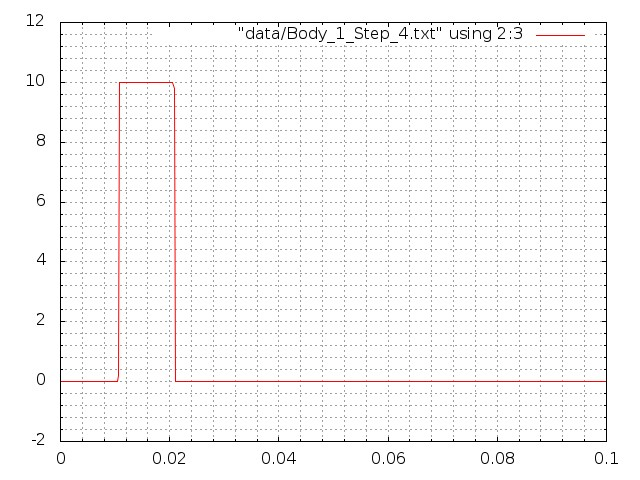
\includegraphics[width=1\linewidth]{png/el-non-mv.png}} a) \\
\end{minipage}
\hfill
\begin{minipage}[h]{0.47\linewidth}
\center{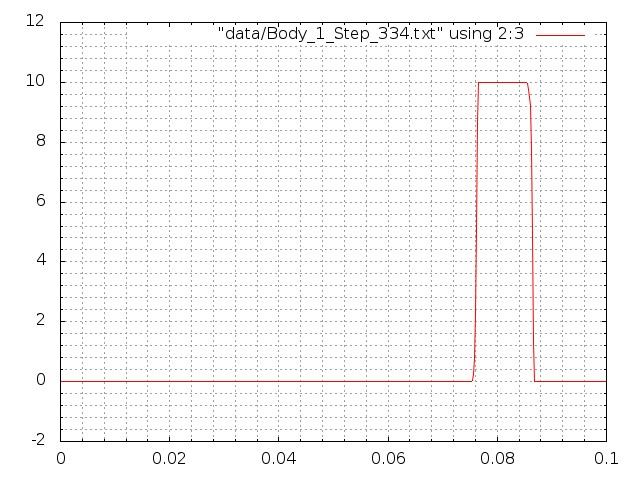
\includegraphics[width=1\linewidth]{png/el-non-mv-2.png}} \\b)
\end{minipage}
\vfill
\begin{minipage}[h]{0.47\linewidth}
\center{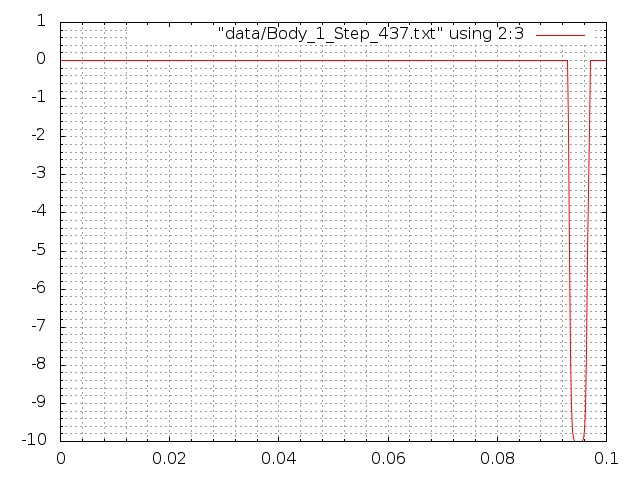
\includegraphics[width=1\linewidth]{png/el-non-mv-2,5.png}} c) \\
\end{minipage}
\hfill
\begin{minipage}[h]{0.47\linewidth}
\center{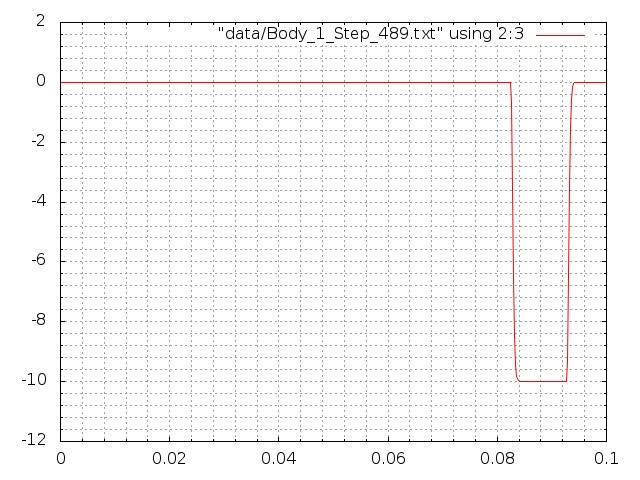
\includegraphics[width=1\linewidth]{png/el-non-mv-3.png}} d) \\
\end{minipage}
\caption{Распространение прямоугольного импульса, неподвижная сетка a) начальное возмущение, b)
импульс прошёл через всё тело, c) отражение от закреплённой границы, d) Отражённый импульс.}
\label{pic:el-non-mv}
\end{figure}

\subparagraph{Подвижная сетка}
В силу равенства нулю правой части и неподвижности сетки вышеизложенный метод абсолютно точен по времени. В случае движения сетки возникают проблемы с порядком точности по времени, которые решаются более симметричным расщеплением процессов распространения возмущения и переноса вещества, описанным в .

На рис.\ref{pic:el-mv} показано отражение упругой волны от свободной границы (граничное условие $\sigma = 0$,       скорость сохраняет знак). Благодаря расщеплению размытие фронта остаётся таким же, как и в методе на неподвижной сетке.

\begin{figure}
\begin{minipage}[h]{0.47\linewidth}
\center{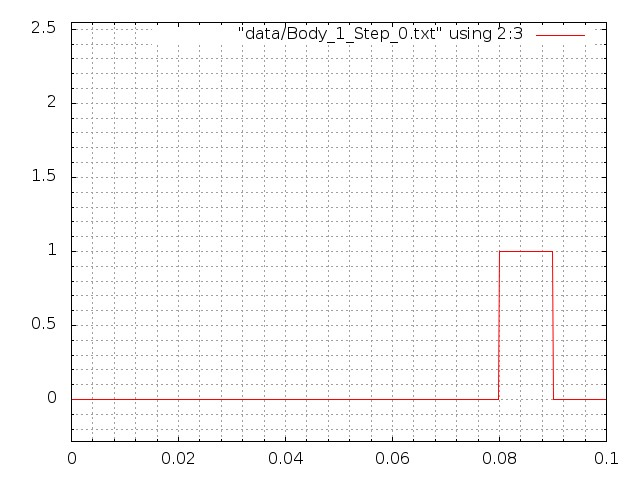
\includegraphics[width=1\linewidth]{png/el-mv.png}} a) \\
\end{minipage}
\hfill
\begin{minipage}[h]{0.47\linewidth}
\center{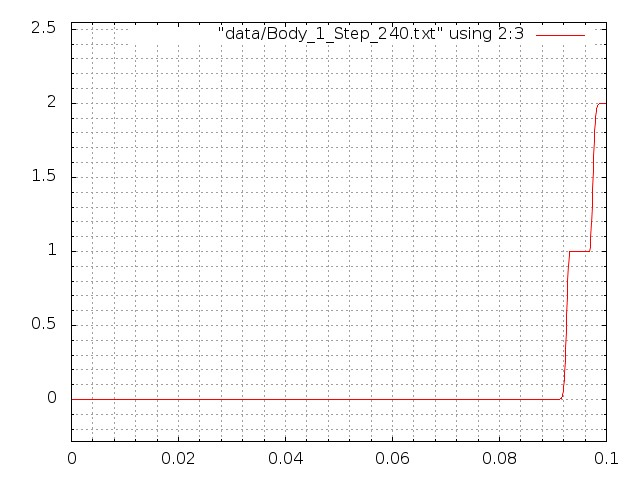
\includegraphics[width=1\linewidth]{png/el-mv-2.png}} \\b)
\end{minipage}
\vfill
\begin{minipage}[h]{0.47\linewidth}
\center{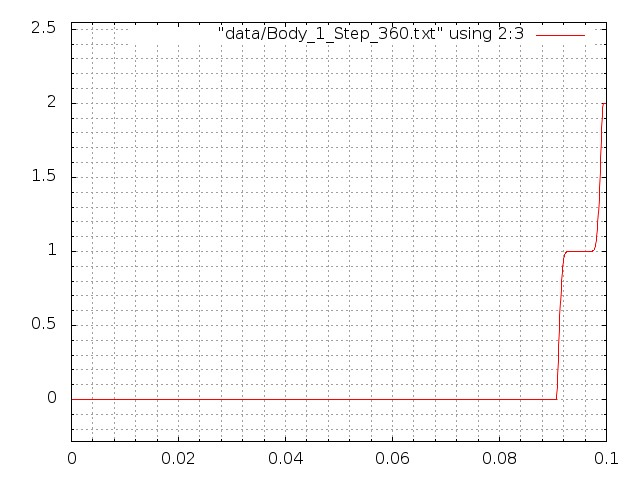
\includegraphics[width=1\linewidth]{png/el-mv-3.png}} c) \\
\end{minipage}
\hfill
\begin{minipage}[h]{0.47\linewidth}
\center{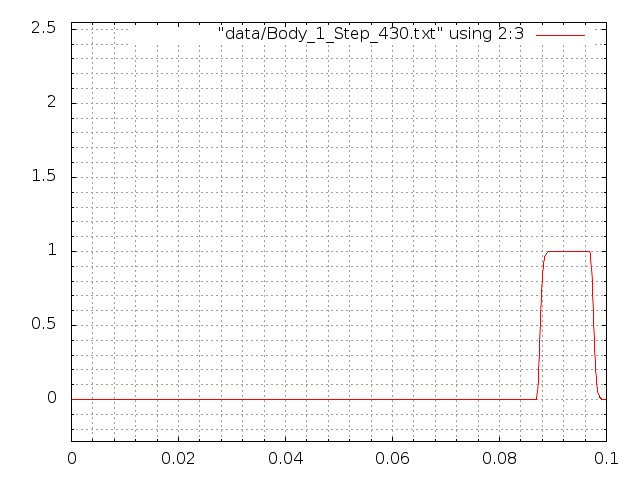
\includegraphics[width=1\linewidth]{png/el-mv-4.png}} d) \\
\end{minipage}
\caption{Распространение прямоугольного импульса, подвижная сетка a) начальное возмущение, b,c) отражение от свободной границы, d) Отражённый импульс.}
\label{pic:el-mv}
\end{figure}

\subparagraph{Ударная волна}
Подвижность сетки позволяет получать гораздо более реальные результаты -- к примеру, в случае достаточно больших скоростей начальных возмущений, независимо от их гладкости, в материале образуется ударная волна (рис.\ref{pic:udarnaya-volna}).

\begin{figure}
\begin{minipage}[h]{0.47\linewidth}
\center{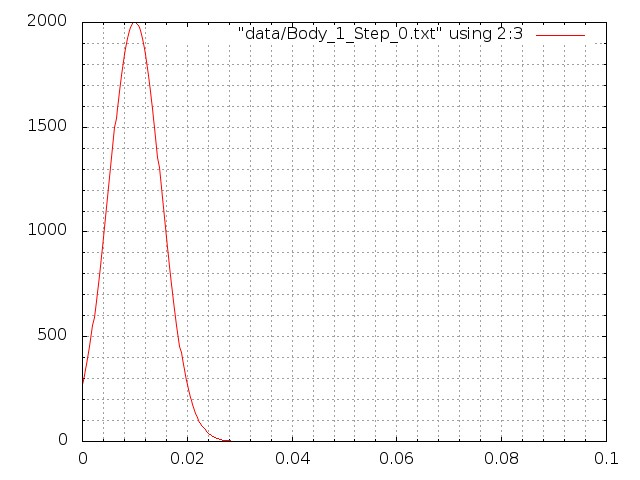
\includegraphics[width=1\linewidth]{png/ud-volna.png}} a) \\
\end{minipage}
\hfill
\begin{minipage}[h]{0.47\linewidth}
\center{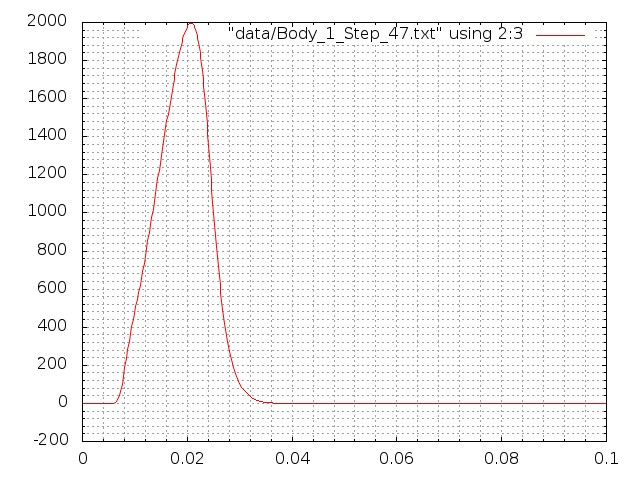
\includegraphics[width=1\linewidth]{png/ud-volna-2.png}} \\b)
\end{minipage}
\vfill
\begin{minipage}[h]{0.47\linewidth}
\center{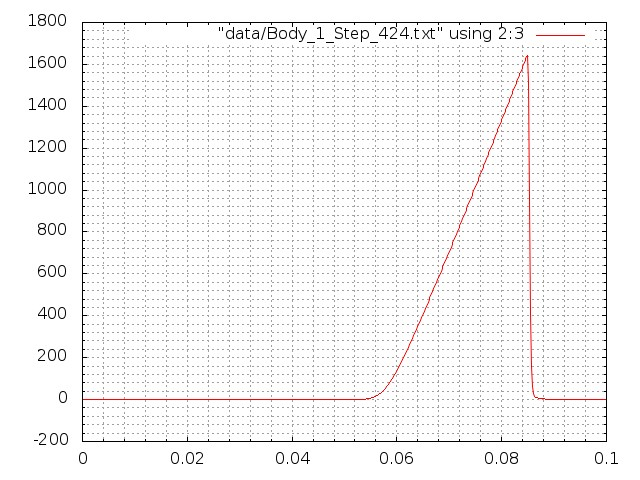
\includegraphics[width=1\linewidth]{png/ud-volna-3.png}} c) \\
\end{minipage}
\hfill
\begin{minipage}[h]{0.47\linewidth}
\center{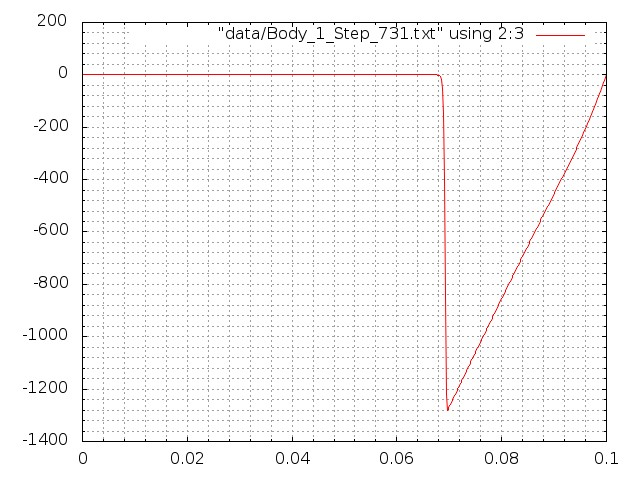
\includegraphics[width=1\linewidth]{png/ud-volna-4.png}} d) \\
\end{minipage}
\caption{Формирование ударной волны при гладком начальном условии a) начальное возмущение - гауссова кривая, b,c) опрокидывание фронта, d) отражённый импульс.}
\label{pic:udarnaya-volna}
\end{figure}

\subparagraph{Рассчёт слоистой структуры}
Также в работе был произведён рассчёт прохождения возмущения через многослойную структуру с возрастающей от слоя к слою плотностью. На рис.\ref{pic:mnogosloika} показаны значения скорости в частицах материала по мере прохождения в новые слои.

\begin{figure}
\begin{minipage}[h]{0.47\linewidth}
\center{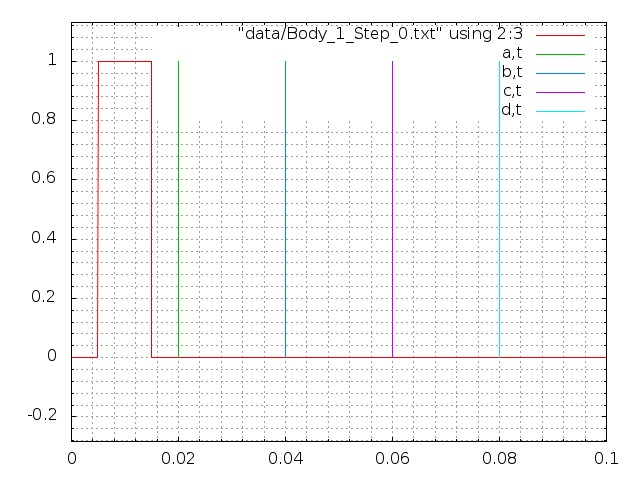
\includegraphics[width=1\linewidth]{png/mnogosloika.png}}  \\
\end{minipage}
\hfill
\begin{minipage}[h]{0.47\linewidth}
\center{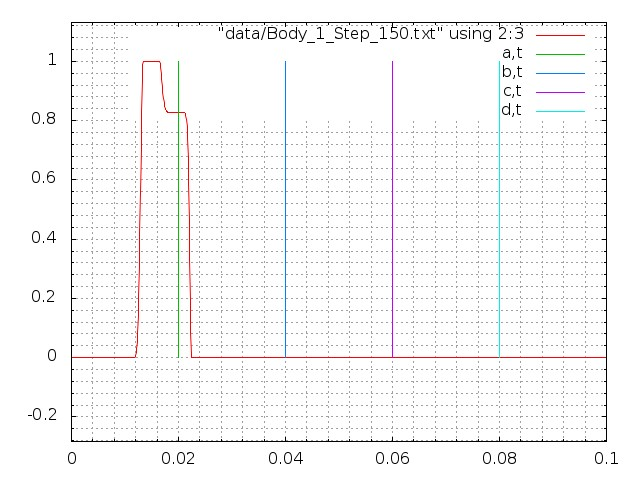
\includegraphics[width=1\linewidth]{png/mnogosloika-2.png}} \\
\end{minipage}
\vfill
\begin{minipage}[h]{0.47\linewidth}
\center{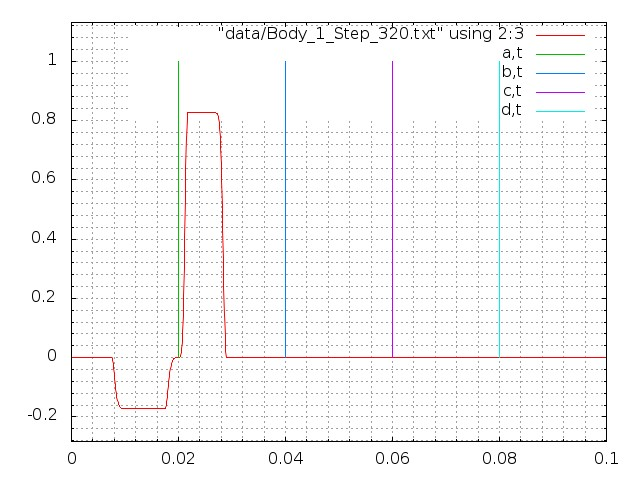
\includegraphics[width=1\linewidth]{png/mnogosloika-3.png}}  \\
\end{minipage}
\hfill
\begin{minipage}[h]{0.47\linewidth}
\center{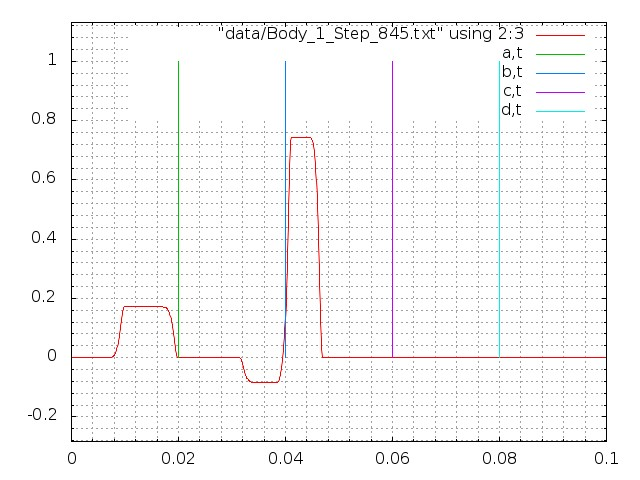
\includegraphics[width=1\linewidth]{png/mnogosloika-4.png}}  \\
\end{minipage}
\vfill
\begin{minipage}[h]{0.47\linewidth}
\center{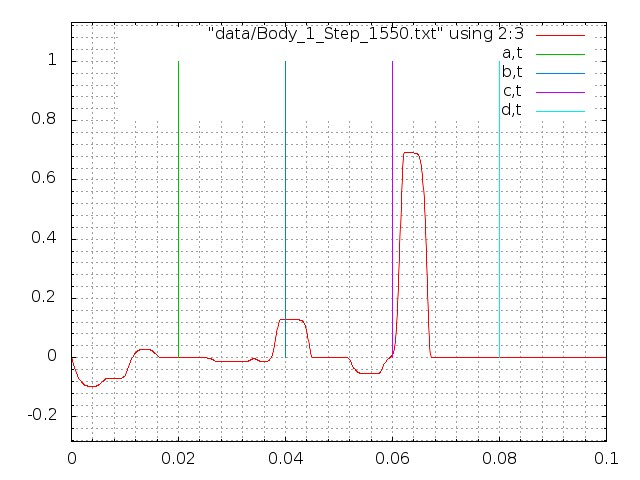
\includegraphics[width=1\linewidth]{png/mnogosloika-5.png}} \\
\end{minipage}
\hfill
\begin{minipage}[h]{0.47\linewidth}
\center{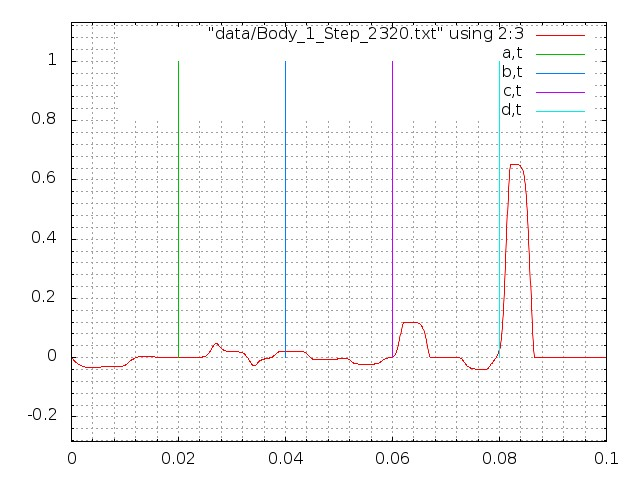
\includegraphics[width=1\linewidth]{png/mnogosloika-6.png}} \\
\end{minipage}
\caption{Прохождение упругой волны через слоистый материал.}
\label{pic:mnogosloika}
\end{figure}

Сравнение численных рассчётов с аналитическими результатами, изложенными в \cite{petrov_tormasov_holodov}, показало их совпадение с высокой (относительная ошибка $10^{-10}$ во втором слое и $10^{-3}$ в пятом) точностью.

\subsubsection{Упругопластика}
Для случая упругопластики в одномерном случае была использована модель с кусочно-линейным по напряжению модулем Юнга (производной $\frac{d\sigma}{d\varepsilon}$) и однозначной зависимостью $\sigma-\varepsilon$. Распространение пластического возмущения показано на рис.\ref{pic:plastic-1d}.

\begin{figure}
\begin{minipage}[h]{0.47\linewidth}
\center{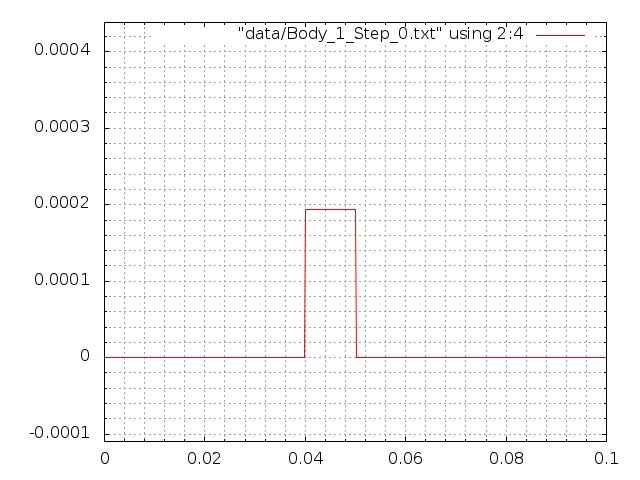
\includegraphics[width=1\linewidth]{png/plastic-1d.png}} a) \\
\end{minipage}
\hfill
\begin{minipage}[h]{0.47\linewidth}
\center{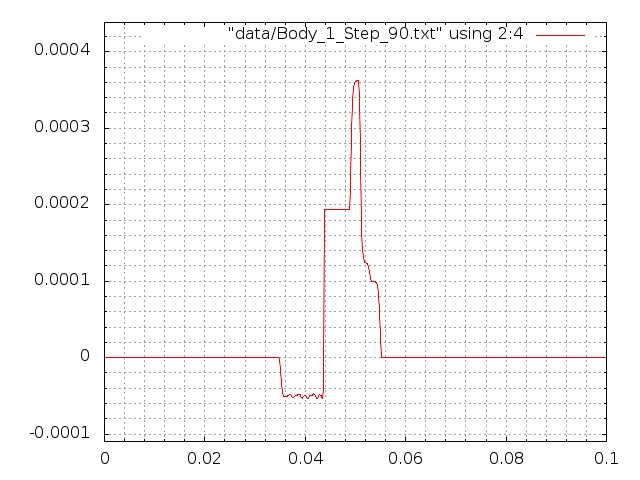
\includegraphics[width=1\linewidth]{png/plastic-1d-2.png}} \\b)
\end{minipage}
\vfill
\begin{minipage}[h]{0.47\linewidth}
\center{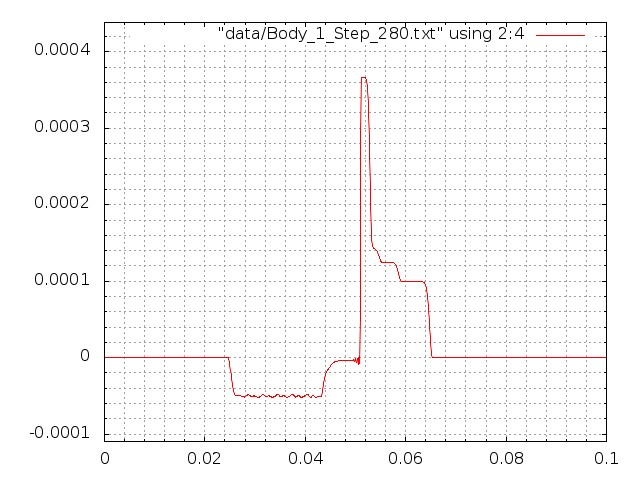
\includegraphics[width=1\linewidth]{png/plastic-1d-3.png}} c) \\
\end{minipage}
\hfill
\begin{minipage}[h]{0.47\linewidth}
\center{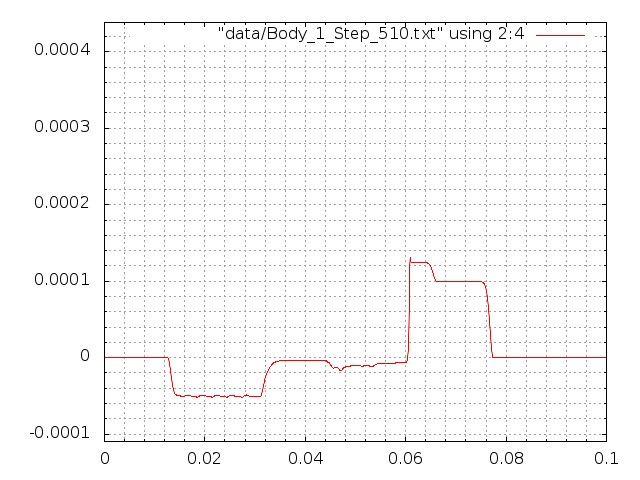
\includegraphics[width=1\linewidth]{png/plastic-1d-4.png}} d) \\
\end{minipage}
\caption{Пластические возмущения a) начальное возмущение - прямоугольник, b) влево уходит чисто упругая волна, справа образуются "упругие предвестники", c) отчётливые четыре "ступеньки" в пластической волне, d) пластическая волна переходит в упругую.}
\label{pic:plastic-1d}
\end{figure}

Четыре "ступеньки" в пластической волне обусловлены четыремя различными значениями модуля Юнга, и, соответственно, скоростями распространения $c = \sqrt{\frac{E}{\rho}}$. Значения напряжений в них совпадают с максимальным верхним пределом, при котором модуль Юнга всё ещё имеет соответствующее значение.

\subsubsection{Неявный метод}
В рамках одномерного кода был также реализован неявный метод второго порядка на неподвижной сетке, описанный в \cite{kukudganov}, стр. 183, являющийся абсолютно устойчивым по времени. Однако практика показала, что он менее пригоден для моделирования динамических процессов ввиду ряда недостатков:
\begin{itemize}
\item Общая сложность реализации, которая вряд ли позволит применить метод в трёхмерном случае
\item Автору неизвестен метод распараллеливания на произвольное число процессов
\item Существенно большее размытие фронтов и величина осцилляций, чем у явного метода второго порядка (см. рис.\ref{pic:implicit})
\item Несмотря на абсолютную устойчивость, при выборе большого шага по времени смоделированная картина перестаёт соответствовать действительности
\end{itemize}
Возможно, данный метод будет полезен для статических рассчётов, в которых не важна кратковременная волновая картина и требуется рассчёт на существенно больших временах.

\begin{figure}
\begin{minipage}[h]{0.47\linewidth}
\center{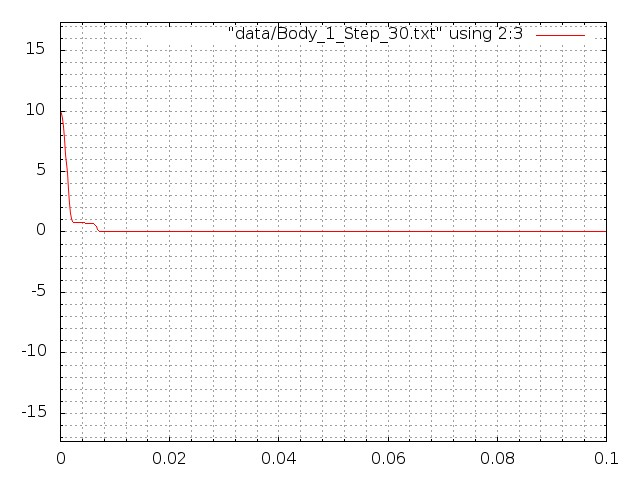
\includegraphics[width=1\linewidth]{png/implicit.png}} \\
\end{minipage}
\hfill
\begin{minipage}[h]{0.47\linewidth}
\center{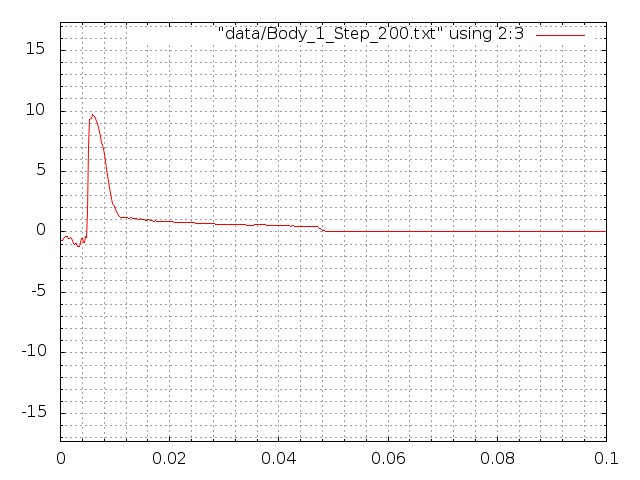
\includegraphics[width=1\linewidth]{png/implicit-2.png}} \\
\end{minipage}
\vfill
\begin{minipage}[h]{0.47\linewidth}
\center{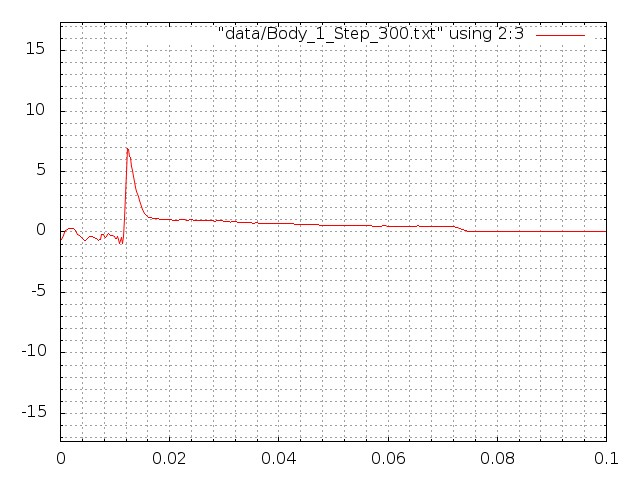
\includegraphics[width=1\linewidth]{png/implicit-3.png}} \\
\end{minipage}
\hfill
\begin{minipage}[h]{0.47\linewidth}
\center{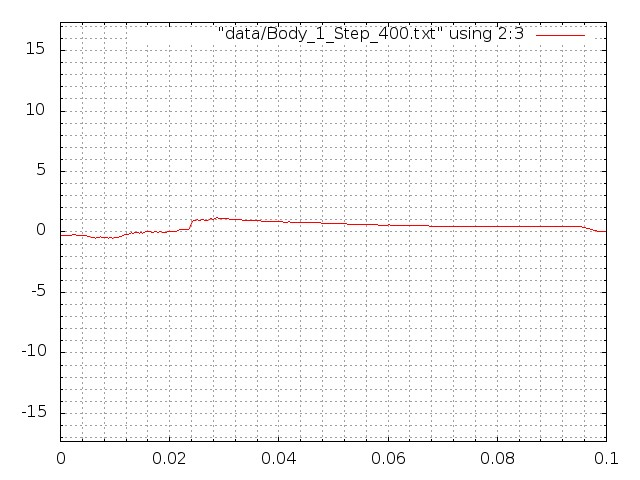
\includegraphics[width=1\linewidth]{png/implicit-4.png}} \\
\end{minipage}
\caption{Боковой удар по телу с пластической реологией. Рассчёт неявным методом второго порядка со сглаживанием}
\label{pic:implicit}
\end{figure}

\subsection{Рассчёты в 3D}